\documentclass[conference]{IEEEtran}
\usepackage{cite}
\usepackage{amsmath}
\usepackage{graphicx}
\usepackage{url}
\usepackage{booktabs}
\usepackage[utf8]{inputenc}

% --- Layout tightening (within IEEE conference style) ---
\setlength{\textfloatsep}{3pt plus 1pt minus 1pt}
\setlength{\intextsep}{3pt plus 1pt minus 1pt}
\setlength{\abovecaptionskip}{1pt}
\setlength{\belowcaptionskip}{0pt}
\setlength{\dbltextfloatsep}{3pt plus 1pt minus 1pt}
\linespread{0.96}

\begin{document}

\title{\large Cross-Attention against Late, FiLM, and Gated Fusion\\for Caption-Guided Land-Cover Understanding}

\author{\IEEEauthorblockN{Süleyman Ceran}
\IEEEauthorblockA{Middle East Technical University\\
Graduate School of Informatics\\
DI 725 -- Transformers and Attention-Based Deep Networks}}

\maketitle

% =============================================================================
% Phase-1 content (kept; describes the original survey, proposal, PoC).
% =============================================================================

\section{Literature Survey}

Vision-language models (VLMs) jointly represent visual and textual information through contrastive learning~\cite{radford2021clip} and have gained traction in remote sensing (RS), where Wen et al.~\cite{wen2024vlm} identify ``cross-modal fusion'' as a major open challenge. RemoteCLIP~\cite{liu2024remoteclip}, the first CLIP for RS, outperforms vanilla CLIP by up to 6.39\% on zero-shot classification via domain-adapted pretraining. Recent multimodal LLMs such as EarthGPT~\cite{zhang2024earthgpt} and RingMoGPT~\cite{wang2025ringmogpt} unify captioning, VQA, grounding, and change detection within a single instruction-tuned framework that projects visual tokens into LLM token spaces.

A central design choice is how to fuse the two modalities. Cross-modal attention has beaten unimodal methods on RS VQA~\cite{bazi2022bimodal} and visual grounding~\cite{lan2024grounding}, and SegCLIP~\cite{zhang2024segclip} fuses text with image features for RS segmentation; FiLM~\cite{perez2018film} offers an attention-free alternative via per-feature affine modulation. Yet few studies directly compare cross-attention against late or feature-wise fusion on RS scene-level tasks, and the effect of caption-generation strategy on fusion performance remains under-explored despite evidence that caption source and quality strongly affect multi-modal models~\cite{chen2024sharegpt4v}.

\section{Project Proposal and Proof of Concept}

\textbf{RQ (Phase-1):} How effective is cross-attention compared to late fusion for RS scene classification with LLM-generated captions? \textbf{Dataset:} ARAS400K~\cite{caglar2026aras400k}---10{,}000 satellite images with 7-class segmentation masks, composition percentages, and 5 captions per image (vision-only, text-only, hybrid); Phase-1 used an 8-class dominant-class label (threshold 50\%). \textbf{Method:} a frozen vanilla CLIP-ViT-B/32 backbone with two trainable heads---late fusion of pooled CLS embeddings and cross-attention with text-as-queries over image patches---across 5 captions $\times$ 2 fusions plus image-only (11 conditions). \textbf{PoC:} 81\% val accuracy on a 500-sample, 5-epoch run (vs.\ 12.5\% chance) confirmed pipeline feasibility.

% =============================================================================
% Phase-2 extension (2-page maximum).
% =============================================================================

\section{Method Refinement}

The Phase-1 review~\cite{phase1feedback} raised three concerns---trivial task, unjustified backbone, insufficient sample size---addressed along three corresponding axes. A pre-experiment confirmed the first: a text-only classifier on the original dominant-class task reaches mAP~$\approx 0.83$ alone, since captions encode the same composition statistics that define the labels. We re-cast the target as 7-bit multi-label class presence with threshold $\tau{=}10\%$, exposing minor classes (Shrub, Built-up, Water, Barren; each $<$11\% of images) where captions are unreliable and image--text complementarity is genuine; we also pilot a patch-level segmentation extension (Path~B, Sec.~\ref{sec:seg}). The frozen backbone is upgraded to RemoteCLIP-ViT-B/32~\cite{liu2024remoteclip}, with forward hooks on \texttt{ln\_post}/\texttt{ln\_final} recovering all 50 patch tokens and 77 text tokens. The fusion comparison expands from 2 to 4: \emph{Late} concatenation $[i\Vert t]$; \emph{FiLM}~\cite{perez2018film} ($i'{=}(1{+}\gamma)\odot i + \beta$, $(\gamma,\beta)$ from pooled text); \emph{Gated} ($g{=}\sigma(W[i\Vert t])$, $g\odot i+(1{-}g)\odot t$); and \emph{Cross-Attention} (CA) with multi-head attention---text tokens query image patches for classification, the direction \emph{inverted} for segmentation. All share a 256-unit ReLU--Dropout--Linear head; only the fusion module and head train.

\section{Experimental Setup}

We use the full 10K ARAS400K corpus, an 80/20 stratified train/val split (stratifying on the dominant class, fixed seed), and 3 random seeds per condition. All conditions train for 30 epochs with AdamW (lr$=10^{-3}$, weight-decay$=10^{-4}$, batch~256/128) using BCE-with-logits (Path~A) or per-patch cross-entropy (Path~B). Best-epoch metrics are reported as mean$\pm$std across the three seeds: mAP, macro F1, and per-class F1 for Path~A; mIoU and per-class IoU for Path~B. With features cached after a single forward pass through the frozen backbone, the entire 117-run matrix (33 Path~A + 33 backbone + 30 fusion-variant + 21 seg) completes in $<$15~min on one A100. All runs are public on Weights \& Biases and the codebase on GitHub~\cite{repo2026phase2}, addressing the Phase-1 reproducibility feedback.

\section{Multi-Label Classification: Results and Ablations}

\begin{figure}[t]
\centering
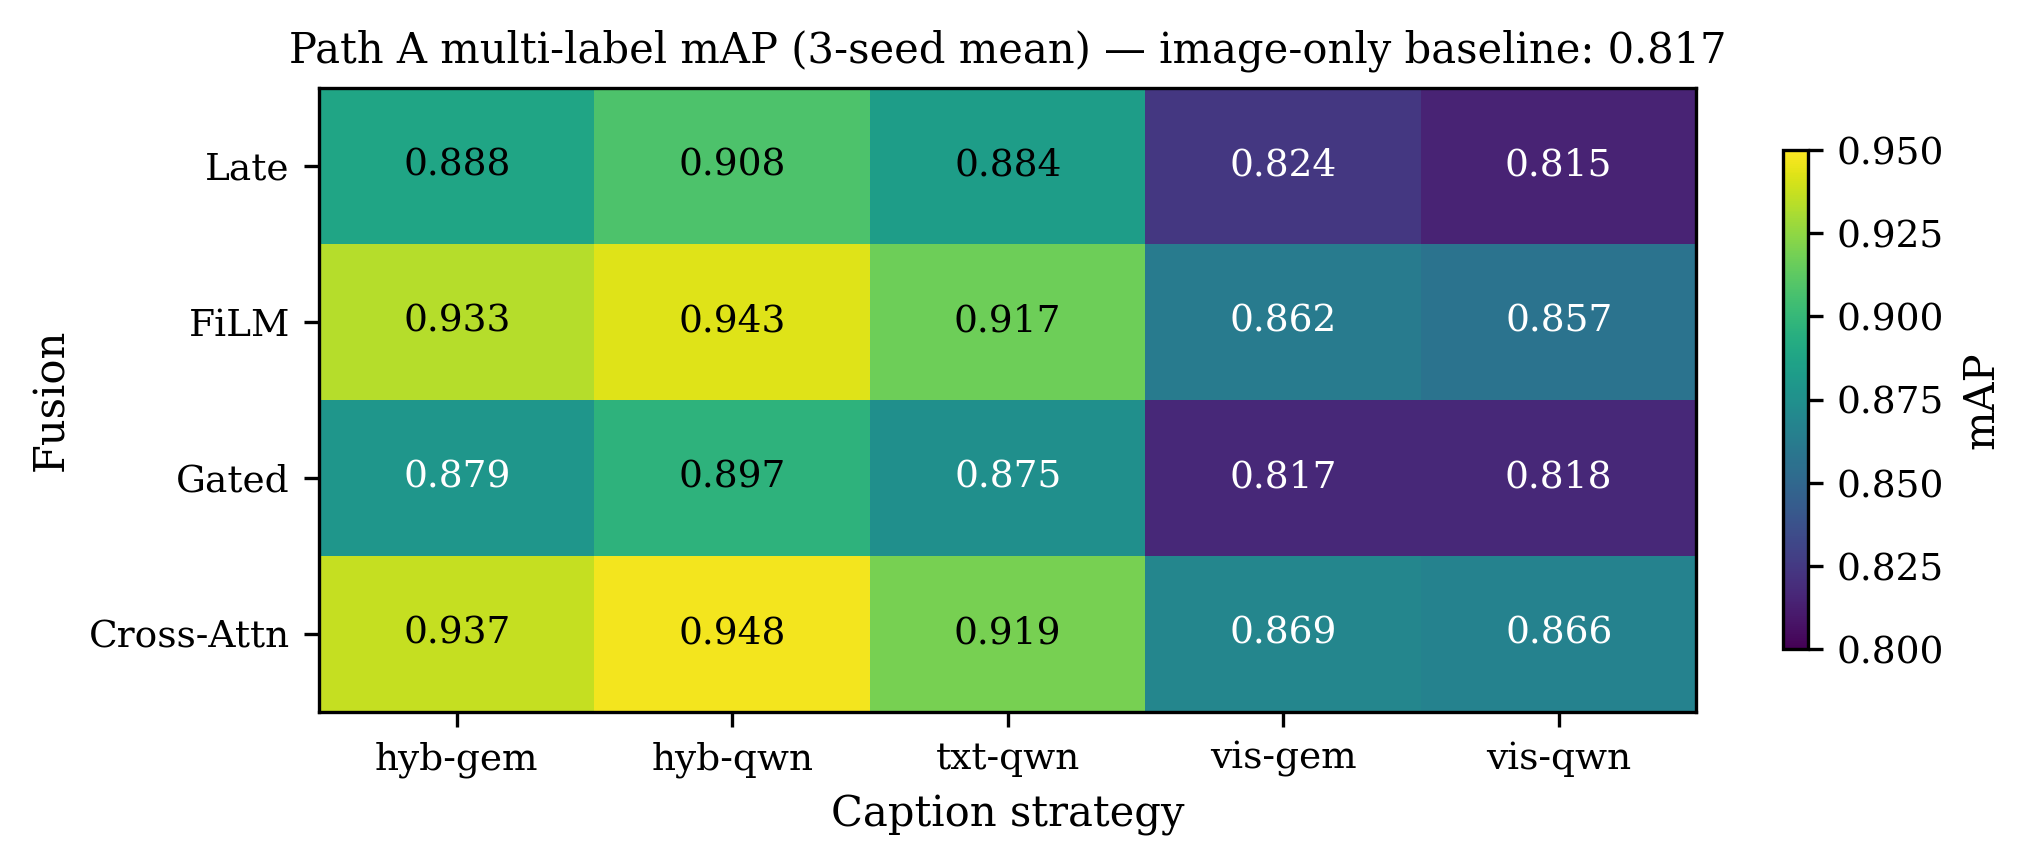
\includegraphics[width=\columnwidth]{figures/fig1_fusion_heatmap.png}
\caption{\footnotesize Path~A multi-label mAP (3-seed mean): fusion (rows) vs.\ caption (cols). Image-only baseline: $0.817\pm0.001$.}
\label{fig:heatmap}
\end{figure}

\textbf{Headline.} Cross-attention with \texttt{hybrid\_qwen3-vl-8b} attains mAP $0.948\pm0.003$ and macro F1 $0.867\pm0.014$, against an image-only baseline of $0.817\pm0.001$---an absolute $+0.131$ mAP gain from caption-guided fusion. Fig.~\ref{fig:heatmap} shows the full $4{\times}5$ matrix; Table~\ref{tab:pathA_summary} the per-family best.

\textbf{CA dominates Late} on every caption ($\Delta$ mAP $=+0.036$ to $+0.051$, std $\leq 0.005$). The gap is largest with the noisy \texttt{vision\_qwen3-vl-8b}: Late gains nothing over image-only ($0.815\approx0.817$), but CA recovers $+0.049$. Vision-only LLM captions frequently \emph{hallucinate} (e.g.\ a 92\%-grass scene labeled ``barren''); CA's attention filters unreliable tokens, while the alternatives cannot.

\textbf{Family ranking (mean mAP across captions):} CA $0.908 >$ FiLM $0.903 >$ Late $0.864 >$ Gated $0.857$. FiLM matches CA within $0.005$ mAP at lower cost; Gated \emph{under}-performs Late as the sigmoid gate collapses one modality (a negative result).

\begin{table}[t]
\centering
\caption{\footnotesize Best Path~A result per fusion family (3-seed mean$\pm$std).}
\label{tab:pathA_summary}
\footnotesize
\setlength{\tabcolsep}{4pt}
\renewcommand{\arraystretch}{0.95}
\begin{tabular}{lccc}
\toprule
Fusion & Best mAP & Macro F1 & Mean mAP \\
\midrule
Image-only           & $0.817\pm0.001$ & $0.702\pm0.006$ & ---     \\
Late                 & $0.908\pm0.003$ & $0.836\pm0.009$ & $0.864$ \\
Gated                & $0.897\pm0.001$ & $0.811\pm0.007$ & $0.857$ \\
FiLM                 & $0.943\pm0.001$ & $0.876\pm0.008$ & $0.903$ \\
\textbf{Cross-Attn}  & $\mathbf{0.948\pm0.003}$ & $\mathbf{0.867\pm0.014}$ & $\mathbf{0.908}$ \\
\bottomrule
\end{tabular}
\end{table}

\textbf{Backbone ablation.} Replacing RemoteCLIP with vanilla CLIP-ViT-B/32~\cite{radford2021clip} on all 33 conditions, RemoteCLIP wins \emph{every} one (mean $\Delta$ mAP $+0.031$, range $+0.014$ to $+0.050$, Table~\ref{tab:summary}). The gap is wider for Late ($+0.04$ to $+0.05$) than CA ($+0.014$ to $+0.029$): strong fusion partly compensates for a weaker backbone, but the best run still pairs RemoteCLIP with CA, consistent with Liu~et~al.'s 6.39\% zero-shot advantage.

\textbf{Per-class decomposition} explains where the gain originates: minor classes that the image-only baseline fails on (Shrub F1 $=0.00$, Built-up $0.65$, Barren $0.61$) recover dramatically under CA (Shrub $0.66$, Built-up $0.79$, Barren $0.79$). Captions and images carry complementary information precisely on these classes; the Phase-1 ``trivial-task'' concern is therefore disproved exactly where it would have mattered.

\section{Preliminary Segmentation Extension}
\label{sec:seg}

\begin{figure}[t]
\centering
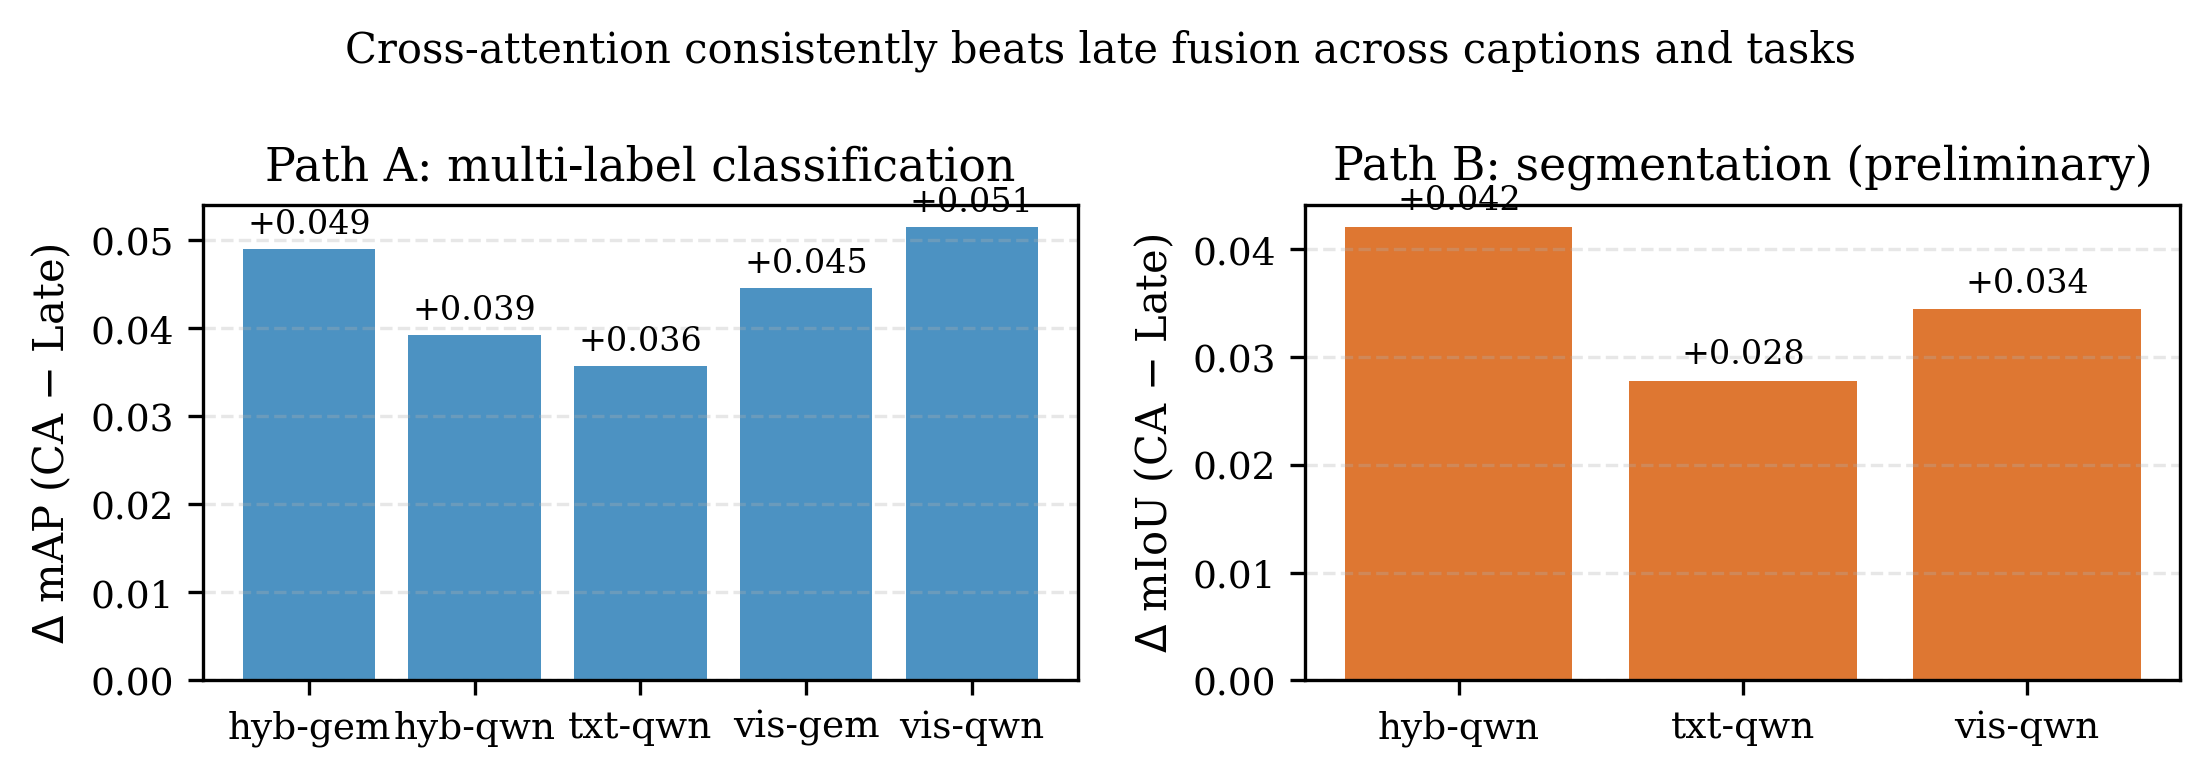
\includegraphics[width=0.95\columnwidth]{figures/fig2_ca_vs_late_delta.png}
\caption{\footnotesize CA-vs-Late advantage across captions, both tasks. Same pattern in classification (left, $\Delta$~mAP) and preliminary segmentation (right, $\Delta$~mIoU); largest gap on the noisy \texttt{vision\_qwen} caption.}
\label{fig:delta}
\end{figure}

The segmentation pipeline reuses cached patch features with two adaptations: the cross-attention direction is \emph{inverted} (image patches query text tokens), and the head outputs per-patch logits over 7 classes; patch-level ground truth is the majority-pool of the $224{\times}224$ mask over each $32{\times}32$ patch (a $7{\times}7$ grid). We run 7 conditions (image-only + 3 captions $\times$ \{late, CA\}) with 3 seeds each.

Best CA segmentation reaches mIoU $0.711 \pm 0.003$ vs.\ image-only $0.574$ ($+0.137$ mIoU, mirroring Path~A's $+0.131$ mAP). CA beats Late on every caption (Fig.~\ref{fig:delta}); the noise-robustness signature persists (Late+\texttt{vision\_qwen} mIoU $0.575 \approx$ image-only; CA+\texttt{vision\_qwen} $0.610$). Per-class IoU shows the largest minor-class lift on Shrub ($0.05\to0.41$, $8\times$), confirming caption guidance contributes spatial localisation signal even where patch-level positives are sparse.

\begin{table}[t]
\centering
\caption{\footnotesize Cross-task summary vs.\ baseline. Both tasks show $\sim{+}0.13$ fusion gain, indicating the CA advantage is not task-specific.}
\label{tab:summary}
\footnotesize
\setlength{\tabcolsep}{4pt}
\renewcommand{\arraystretch}{0.95}
\begin{tabular}{lccc}
\toprule
Setting & Baseline & Best CA & $\Delta$ \\
\midrule
Path~A classification (mAP)              & $0.817$        & $\mathbf{0.948}$ & $+0.131$ \\
Path~B segmentation (mIoU)               & $0.574$        & $\mathbf{0.711}$ & $+0.137$ \\
Backbone (mean mAP, 5 caps)              & $0.840$ (vCLIP)& $0.871$ (RC)     & $+0.031$ \\
\bottomrule
\end{tabular}
\end{table}

\section{Discussion and Phase-3 Outlook}

Three findings emerge. First, \textbf{CA universally beats alternative fusions} on this benchmark: it wins every head-to-head across $4\,\text{fusion}\times 5\,\text{caption}\times 3\,\text{seed}$ in classification and the seg subset, with statistically negligible variance. Second, \textbf{CA's selectivity yields noise robustness}: vision-only LLM captions hallucinate on this dataset, which Late and Gated cannot filter, but cross-attention's weights effectively downweight unreliable tokens (CA recovers $+0.049$ mAP on noisy captions where Late gains nothing). Third, \textbf{the fusion-gain pattern transfers across tasks}: both classification and segmentation show $\sim{+}0.13$ absolute gain over image-only baselines (Table~\ref{tab:summary}), suggesting the result is not specific to scene-level prediction. The Phase-1 ``trivial-task'' concern is therefore addressed empirically: per-class, fusion is most valuable precisely on the minor classes captions describe inconsistently (Shrub F1 $0.00\to0.66$; Shrub IoU $0.05\to0.41$).

All gains are with a frozen backbone; the rank order is stable across captions, seeds, and tasks. Phase-3 will extend the seg matrix to all captions $\times$ 4 fusions, ablate $\tau$ and patch resolution (B/16, $14{\times}14$), and explore parameter-efficient fine-tuning.

\scriptsize
\setlength{\IEEEilabelindent}{0pt}
\setlength{\IEEEiednormlabelsep}{0pt}
\renewcommand{\IEEEbibitemsep}{0pt plus 0.3pt}
\begin{thebibliography}{10}

\bibitem{radford2021clip}
A.~Radford \emph{et al.}, ``Learning transferable visual models from natural language supervision,'' \emph{ICML}, 2021.

\bibitem{wen2024vlm}
C.~Wen \emph{et al.}, ``Vision-Language Models in Remote Sensing,'' \emph{IEEE Geosci.\ Remote Sens.\ Mag.}, vol.~12, 2024.

\bibitem{liu2024remoteclip}
F.~Liu \emph{et al.}, ``RemoteCLIP: A Vision Language Foundation Model for Remote Sensing,'' \emph{IEEE TGRS}, vol.~62, 2024.

\bibitem{zhang2024earthgpt}
W.~Zhang \emph{et al.}, ``EarthGPT: A Universal Multimodal Large Language Model for Multisensor Image Comprehension in Remote Sensing,'' \emph{IEEE TGRS}, vol.~62, 2024.

\bibitem{wang2025ringmogpt}
P.~Wang \emph{et al.}, ``RingMoGPT: A Unified Remote Sensing Foundation Model for Vision, Language, and Grounded Tasks,'' \emph{IEEE TGRS}, vol.~63, 2025.

\bibitem{bazi2022bimodal}
Y.~Bazi \emph{et al.}, ``Bi-Modal Transformer-Based Approach for Visual Question Answering in Remote Sensing Imagery,'' \emph{IEEE TGRS}, vol.~60, 2022.

\bibitem{lan2024grounding}
M.~Lan \emph{et al.}, ``Language Query-Based Transformer for Visual Grounding on Remote Sensing Images,'' \emph{IEEE TGRS}, vol.~62, 2024.

\bibitem{zhang2024segclip}
S.~Zhang \emph{et al.}, ``SegCLIP: Multimodal Visual-Language and Prompt Learning for RS Semantic Segmentation,'' \emph{IEEE TGRS}, vol.~62, 2024.

\bibitem{perez2018film}
E.~Perez \emph{et al.}, ``FiLM: Visual reasoning with a general conditioning layer,'' \emph{AAAI}, 2018.

\bibitem{chen2024sharegpt4v}
L.~Chen \emph{et al.}, ``ShareGPT4V: Improving Large Multi-Modal Models with Better Captions,'' \emph{ECCV}, 2024.

\bibitem{caglar2026aras400k}
M.~Caglar, ``ARAS400K Remote Sensing Dataset,'' Zenodo, 2026, \url{https://zenodo.org/records/18890661}.

\bibitem{phase1feedback}
Phase-1 instructor review, DI~725 Term Project, Spring~2026.

\bibitem{repo2026phase2}
S.~Ceran, ``ARAS multi-modal attention land-cover classification,'' GitHub, 2026, \url{https://github.com/sceran/aras-multimodal-attention-landcover-classification}.

\end{thebibliography}

\end{document}
